\documentclass[a4paper,10pt]{report}
\usepackage[utf8]{inputenc}
\usepackage{graphicx}
%\usepackage[a4paper, total={6in, 8in}]{geometry}

% Title Page
\title{\textbf{OPTICAL COMMUNICATION COMPONENTS \\ Lab 5}}
\author{Nicola Simoni, Tadewos Somano, Melkamsew Tenaw}
\date{University of Brescia, Faculty of Engineering\\A.Y. 2013-2014}


\begin{document}
\maketitle


%%%%%%%%%%%%%%%%%%%%%%%%%%%%%%%%%%%%%%%%%%%%%%%%%%%%%%%%%%%%%%%%%%%%%%%%%%%%%%%%%%%%%%%%%%%%%
\section*{Exercise 1}
We calculate the Rayleigh backscattering power for a standard single mode fiber using the following parameters:
\begin{itemize}
 \item $P_{in} = 1 \ mW$
 \item $\alpha_{dB} = 0.2 \ [dB/Km]$
 \item $L >> \alpha_{dB}$
\end{itemize}

As $L >> \alpha_{dB}$ we can compute the Rayleigh backscattering power using the simplified equation:
$$P_{RS}[dBm]=P_{in}[dBm]+10 \log \left( \frac{\eta}{2 \alpha} \right)$$

$\eta$ is the Rayleigh backscattering coefficient and its value is: $\eta = 4.9034\cdot 10^{-8} \ [1/m]$.
The attenuation must be linear and expressed in [1/m] as well, so we convert it:
$$ \alpha = \log \left( 10^{\frac{\alpha_{dB}}{10}} \right) = \log \left( 10^{\frac{0.2 \cdot 10^{-3}}{10}} \right)= 4.6052\cdot 10^{-5} \ [1/m]$$

The input power must be expressed in dBm and one milliwatt corresponds to 0 dBm.
So we find:
$$P_{RS}[dBm]= 0 + 10 \log \left( \frac{4.9034\cdot 10^{-8}}{2 \cdot 4.6052\cdot 10^{-5}} \right)= -32.7378 \ dBm$$

%%%%%%%%%%%%%%%%%%%%%%%%%%%%%%%%%%%%%%%%%%%%%%%%%%%%%%%%%%%%%%%%%%%%%%%%%%%%%%%%%%%%%%%%%%%%%
\section*{Exercise 2}
Now we run the simulation in order to compare the results with the calculation of Exercise 1.
The parameters are the same as before. We measure the Rayleigh backscattering power for different fiber lengths, starting from 1 Km up to 100 Km, with
steps of 10 Km. In Figure \ref{es2} is shown the result.

\begin{figure}[!ht]
  \centering
  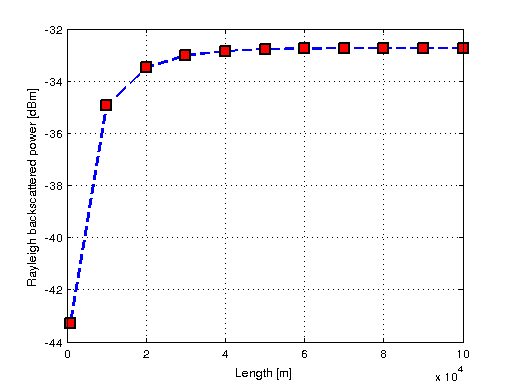
\includegraphics[width=12cm]{es2.png}\\
  \caption{Rayleigh backscattered power versus fiber length.}
  \label{es2}
\end{figure}

The final value on the graph coincides with the computed one.
We can notice that, after a certain length, the Rayleigh backscattered power saturates.
This is due to the fact that the attenuation decreases exponentially with the distance: the
backscattered power that reaches the receiver is only the one due to the first kilometers of propagation.
The power saturates after the effective length of the fiber, that is: $$L_{eff}=\frac{1-e^{-\alpha L}}{\alpha}=5 \cdot 10^3 \ m$$


\newpage
%%%%%%%%%%%%%%%%%%%%%%%%%%%%%%%%%%%%%%%%%%%%%%%%%%%%%%%%%%%%%%%%%%%%%%%%%%%%%%%%%%%%%%%%%%%%%
\section*{Exercise 3}
Following are reported the spectra of the signal at the beginning and at the end of the fiber. The deltas represent Rayleigh distortion and
we can notice that, at the end of the propagation, distortion is increased.

\begin{figure}[!ht]
  \centering
  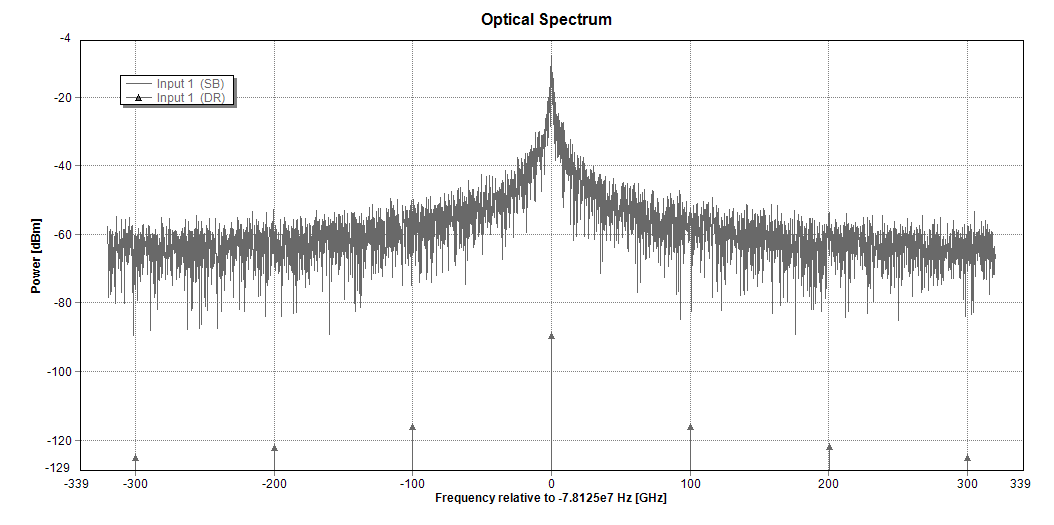
\includegraphics[width=11cm]{es3_1km.png}\\
  \caption{Signal spectrum at 1 Km.}
  \label{es3_1}
\end{figure}

\begin{figure}[!ht]
  \centering
  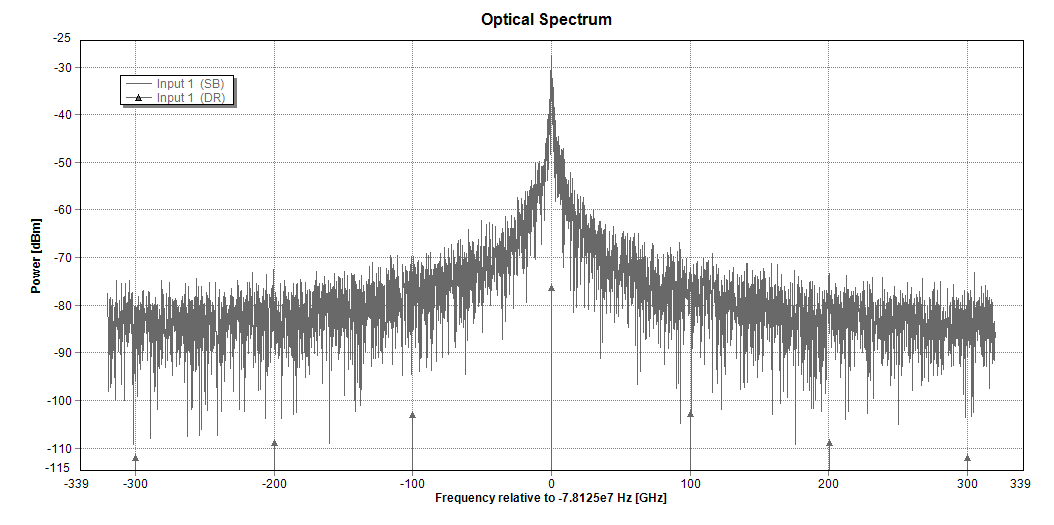
\includegraphics[width=11cm]{es3_100km.png}\\
  \caption{Signal spectrum at 100 Km.}
  \label{es3_2}
\end{figure}


%%%%%%%%%%%%%%%%%%%%%%%%%%%%%%%%%%%%%%%%%%%%%%%%%%%%%%%%%%%%%%%%%%%%%%%%%%%%%%%%%%%%%%%%%%%%%
\section*{Exercise 4}
We scan the Rayleigh scattering coefficient between -80 dB and -52 dB, with steps of 2 dB, and we measure the relative BER.
In Figure \ref{es4} is shown the result.
We want to know for which Rayleigh scattering coefficient the BER exceeds $10^{-9}$, after 80 Km of fiber.
To do this, we zoom the obtained graph around the value -9 (BER is in logarithmic scale) and we read the corresponding value that is nearly -58.23 dB.
After this value the BER starts exceeding the limit value.
In Figure \ref{es4zoom} is shown the measure result.

\begin{figure}[!h]
  \centering
  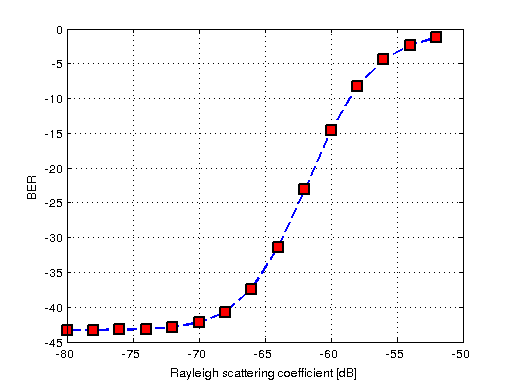
\includegraphics[width=12cm]{es4.png}\\
  \caption{BER versus Rayleigh scattering coefficient.}
  \label{es4}
\end{figure}

\begin{figure}[!h]
  \centering
  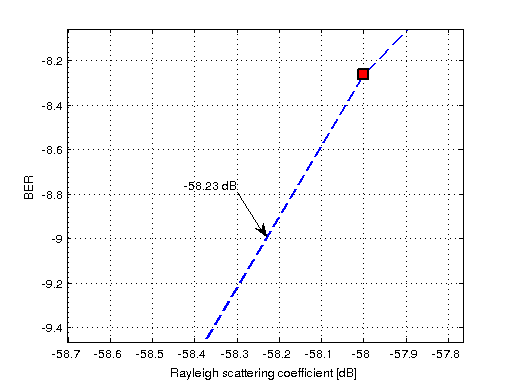
\includegraphics[width=12cm]{es4zoom.png}\\
  \caption{BER versus Rayleigh scattering coefficient, limit value.}
  \label{es4zoom}
\end{figure}


\newpage
%%%%%%%%%%%%%%%%%%%%%%%%%%%%%%%%%%%%%%%%%%%%%%%%%%%%%%%%%%%%%%%%%%%%%%%%%%%%%%%%%%%%%%%%%%%%%
\section*{Exercise 5}
Two optical On Off Keying transmitters, separated by 13 THz, transmit different bit sequences. They both have a power of 10 mW, same phase and
they use the same fiber (that has zero dispersion). At the end of the fiber, using a demultiplexer, the two signals are separated and visualized (the first
channel in grey and the second in red). In Figure \ref{es5} is shown the simulation result.
The value represented by logical ``1'' corresponds to 0.01 on the graph, while the value of ``0'' corresponds to 0.
In the received sequence we notice that we also have two different values: $\approx 0.015$ and $\approx 0.004$.
These values are found when the pulses of the two channels are transmitted in the same instant. In this case, 
the pulses travel overlapped and they experience Raman gain effect, that is, one pulse gives some of its power to the other pulse, amplifying it.
When instead, the pulses are transmitted once at time, they are correctly received.

\begin{figure}[!ht]
  \centering
  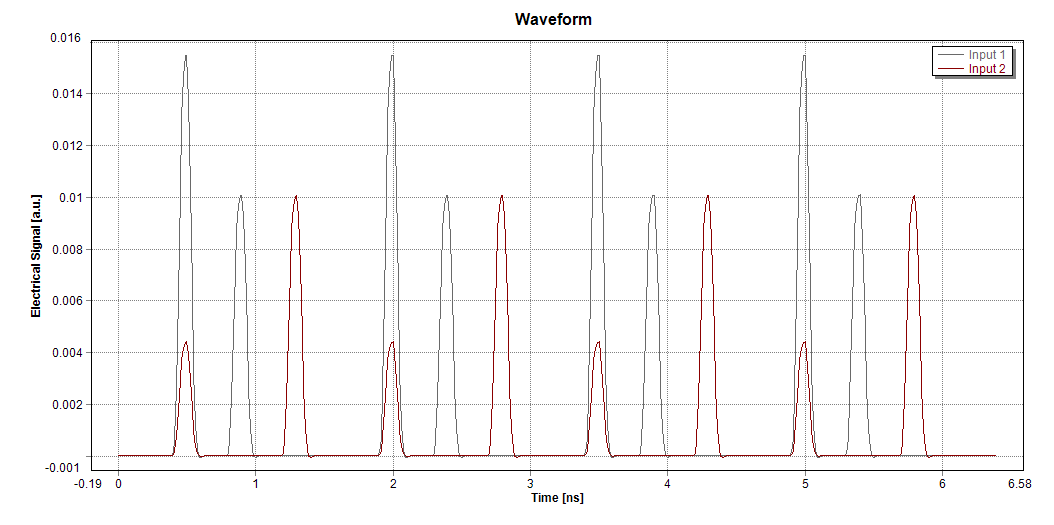
\includegraphics[width=11cm]{es5.png}\\
  \caption{Transmission of pulses in phase.}
  \label{es5}
\end{figure}

\newpage
%%%%%%%%%%%%%%%%%%%%%%%%%%%%%%%%%%%%%%%%%%%%%%%%%%%%%%%%%%%%%%%%%%%%%%%%%%%%%%%%%%%%%%%%%%%%%
\section*{Exercise 6}
We run the same simulation of Exercise 5, but this time, we change the phase (azimuth) of one of the two transmitters by 90 degrees.
In Figure \ref{es6} is shown the simulation result. Now we can notice that the pulses are always correctly received.
This is due to the fact that the two signals are orthogonal and the Raman scattering is polarization dependent.
In this case, the effect is one order of magnitude smaller respect to the case of co-polarization.

\begin{figure}[!ht]
  \centering
  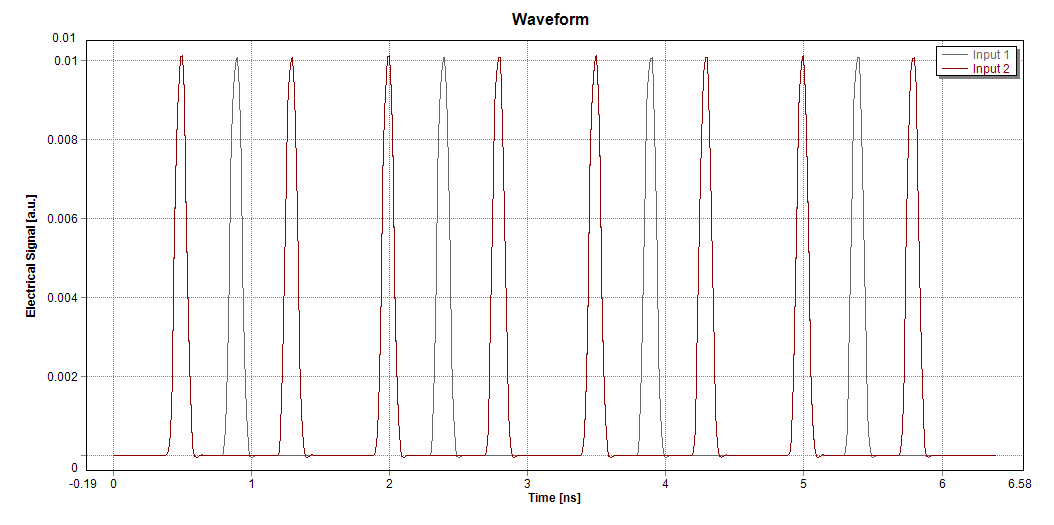
\includegraphics[width=11cm]{es6.png}\\
  \caption{Transmission of pulses with a phase difference of $90^{\circ}$.}
  \label{es6}
\end{figure}


\newpage
%%%%%%%%%%%%%%%%%%%%%%%%%%%%%%%%%%%%%%%%%%%%%%%%%%%%%%%%%%%%%%%%%%%%%%%%%%%%%%%%%%%%%%%%%%%%%
\section*{Exercise 7}
We run the simulation by scanning the input power between -20 dBm and +20 dBm. For each power we measure the transmitted power and the Stokes power,
in Figure \ref{es7} is shown the result. Taking a measure from the graph we find a Brillouin threshold of approximately 7.71 dBm. 

\begin{figure}[!ht]
  \centering
  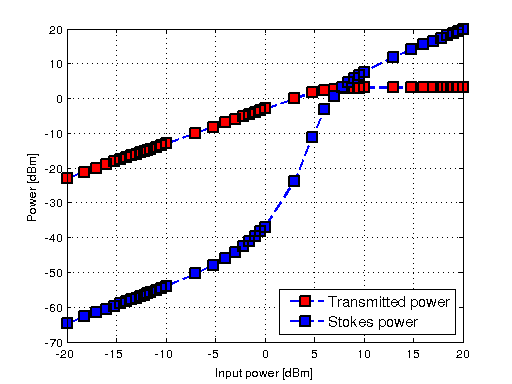
\includegraphics[width=12cm]{es7.png}\\
  \caption{Transmitted power and Stokes power.}
  \label{es7}
\end{figure}

We can compute the analytical value of the Brillouin threshold, by using the following equation:
\begin{equation}\label{pth}
P_{th}\approx21\frac{K A_{eff}}{g_B L_{eff}} \frac{\Delta f_B\otimes \Delta f_P}{\Delta f_B} 
\end{equation}

we substitute in equation (\ref{pth}) the following values:
\begin{itemize}
 \item K=1
 \item $A_{eff}=80 \cdot 10^{-12} \ m^2$
 \item $g_B=2\cdot 10^{-11} \ m/W$
 \item $L_{eff}=1.0832 \cdot 10^{4} \ m$
 \item $\Delta f_B=35\ MHz$
 \item $\Delta f_P=0$
\end{itemize}

and we find:
$$P_{th}\approx 8.89 \ dBm$$

as the equation is approximated, the computed threshold is slightly different respect to the one found with the simulation.

\newpage
%%%%%%%%%%%%%%%%%%%%%%%%%%%%%%%%%%%%%%%%%%%%%%%%%%%%%%%%%%%%%%%%%%%%%%%%%%%%%%%%%%%%%%%%%%%%%
\section*{Exercise 8}
Now we modulate a continuous wave signal using a phase modulator with parameters f=2 GHz and $\Delta \Phi = 180^{\circ}$.
We vary the input power from -20 dBm to +20 dBm and we measure the Stokes power: in Figure \ref{es8} is shown the simulation result.
The Brillouin threshold is nearly 16.59 dBm. It is increased by 8.88 dBm respect to the case without phase modulation.
This is due to the fact that now the term $\Delta f_P$ in equation (\ref{pth}) is no more zero, and so the value $P_{th}$ increases.

\begin{figure}[!ht]
  \centering
  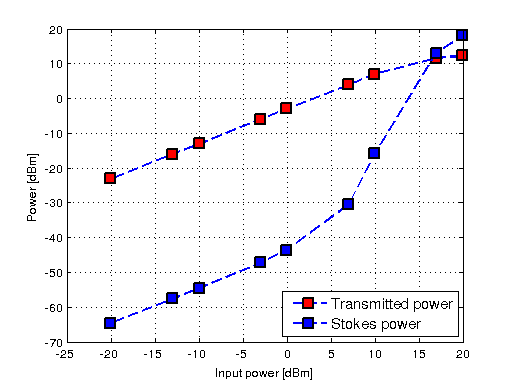
\includegraphics[width=12cm]{es8.png}\\
  \caption{Transmitted power and Stokes power.}
  \label{es8}
\end{figure}


\newpage
%%%%%%%%%%%%%%%%%%%%%%%%%%%%%%%%%%%%%%%%%%%%%%%%%%%%%%%%%%%%%%%%%%%%%%%%%%%%%%%%%%%%%%%%%%%%%
\section*{Exercise 9}
We have to compute the phase value for which the maximal Brillouin scattering power is -10 dBm.
We compute the Stokes and transmitted power for different phase values.
In Figure \ref{es9} is shown the simulation result. From the graph we can deduce that, to satisfy the condition, the phase has to be:
$$|\Phi|>132.7^{\circ}$$

\begin{figure}[!ht]
  \centering
  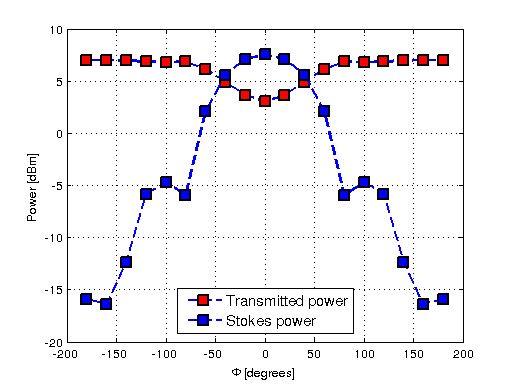
\includegraphics[width=12cm]{es9.png}\\
  \caption{Transmitted power and Stokes power.}
  \label{es9}
\end{figure}

\end{document}